
\section{Functional Magnetic Resonance Imaging}

As established the BOLD contrast is effected by the neural activity producing changes in the local blood flow, blood volume and blood oxygenation. These metabolic changes associated with different neurological tasks can be accentuated through the use of fMRI \cite{Glover2011}. The following section will introduce the concept of fMRI and why it can be used to study brain activation. Before reading this section, it is assumed that the reader is familiar with basic physics of nuclear magnetic resonance imaging and image reconstruction. If not, an overview can be found appendices \ref{sec:physics} and \ref{sec:IMrec}. 

The fundamental reason to why fMRI can used to study brain activity relies on the indirect measure of the magnetic properties of Blood. MRI is dependent on susceptibility, which is the extend to which a material can be affected by magnetization. Local changes in susceptibility results in changes in the MRI signal. \cite{Syed2015} Changes in susceptibility arise with the hemodynamic response as oxygenated hemoglobin $(HbO_2)$ is diamagnetic, and deoxygenated hemoglobin $(Hb)$ is highly paramagnetic due to its four unpaired electrons, resulting in what is known as the Blood Level Oxygen Dependent (BOLD) contrast. Thus, as presented in the prior section, the increase in neural activity increases the blood flow to an extend greater than metabolic utilization of oxygen resulting in high  $(HbO_2)$ to $(Hb)$ ratio, the BOLD contrast. \cite{Glover2011,Poldrack2011,Khanna2015} \Figref{fig:back:bold} illustrates how the BOLD contrast is dependent on the amount of oxygenated hemoglobin. 

\begin{figure}[H]                 
	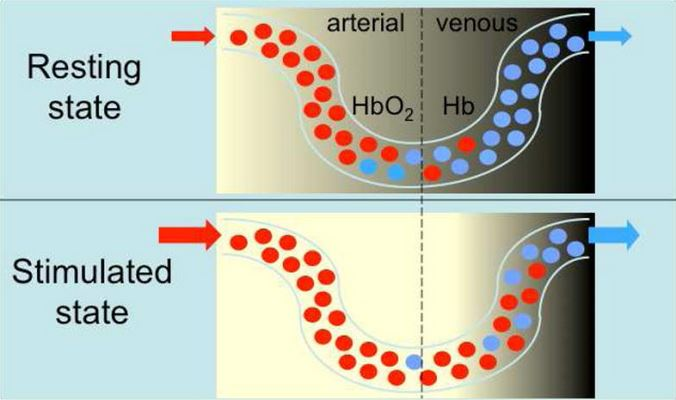
\includegraphics[width=.47\textwidth]{figures/aBackground/bold_response}  
	\caption{Illustration of how the difference in oxygen concentration in the hemoglobin change the magnetic properties, resulting in a higher measurable contrast \cite{Glover2011}.}
	\label{fig:back:bold} 
\end{figure}

The changes in the BOLD contrast can be recorded by using a $T2^*$ sequence, which is sensitive in detecting changes on the magnetic field \cite{Khanna2015,Lee2002}. The areas highly filled with oxygenated blood will result in bigger signal in the $T2^*$ wighted sequence making these are brighter in the reconstructed image. To capture the changes in blood flow over time the acquisitions has to be relatively fast. To achieve fast sequences, the result is a sacrifice of spatial resolution for temporal resolution, making it possible to acquire a whole brain volume in a couple of seconds. \cite{Khanna2015} \\ 
Other methods, as the arterial spin labeled (ASL) method exist for accentuating the functionality of the brain, but BOLD is favored, because it offers a high contrast to noise ratio and it is relatively simple to implement. \cite{Lee2002}    
